%----------------------------------------------------------------------------------------
%	PACKAGES AND OTHER DOCUMENT CONFIGURATIONS
%----------------------------------------------------------------------------------------

\documentclass[a0paper,portrait]{baposter}

\usepackage[font=small,labelfont=bf]{caption} % Required for specifying captions to tables and figures
\usepackage{booktabs} % Horizontal rules in tables
\usepackage{relsize} % Used for making text smaller in some places

\usepackage{amsmath,amsfonts,amssymb,amsthm} % Math packages
\usepackage{eqparbox}

\usepackage{textcomp}

\usepackage[brazil]{babel}
\usepackage[utf8]{inputenc}

\usepackage{wrapfig}

\graphicspath{{figures/}} % Directory in which figures are stored

 \definecolor{bordercol}{RGB}{45, 235, 118} % Border color of content boxes
 \definecolor{headercol1}{RGB}{5, 184, 255} % Background color for the header in the content boxes (left side)
 \definecolor{headercol2}{RGB}{26, 167, 85} % Background color for the header in the content boxes (right side)
 \definecolor{headerfontcol}{RGB}{0, 0, 0} % Text color for the header text in the content boxes
 \definecolor{boxcolor}{RGB}{255, 255, 255} % Background color for the content in the content boxes


\begin{document}

\background{% Set the background to an image (background.pdf)
\begin{tikzpicture}[remember picture,overlay]
\draw (current page.north west)+(-2em,2em) node[anchor=north west]
{
\includegraphics[height=1.1\textheight]{background}};
\end{tikzpicture}
}

\begin{poster}
{grid=false,
borderColor=bordercol, % Border color of content boxes
headerColorOne=headercol1, % Background color for the header in the content boxes (left side)
headerColorTwo=headercol2, % Background color for the header in the content boxes (right side)
headerFontColor=headerfontcol, % Text color for the header text in the content boxes
boxColorOne=boxcolor, % Background color for the content in the content boxes
headershape=roundedright, % Specify the rounded corner in the content box headers
headerfont=\Large\sf\bf, % Font modifiers for the text in the content box headers
textborder=rectangle,
background=user,
headerborder=open, % Change to closed for a line under the content box headers
boxshade=plain
}
{\begin{tabular}{c}
        
\includegraphics[height=1cm]{UNIVAP-SF.png}\\
\end{tabular}
}
%
%----------------------------------------------------------------------------------------
%	TITLE AND AUTHOR NAME
%----------------------------------------------------------------------------------------
%
{\bf  \LARGE {DECIMETRIC RADIO EMISSION ANALYSIS OF CHROMOSPHERIC EVAPORATION IN A X1.0 FLARE ON MARCH 29, 2014} \\ % Poster title
\vspace{0.2cm}
\footnotesize \underline{André Rossi Korol}, Francisco Carlos Rocha Fernandes\\  % Author names
\footnotesize \it UNIVAP --- Universidade do Vale do Paraíba\\ % Institution names
\footnotesize \it \textcolor{blue}{\underline{anrobits@yahoo.com.br}}\/}
%Author email addresses

{\begin{tabular}{c}
        
\includegraphics[height=1cm]{ipd2-sf.png}
\end{tabular}
}

%----------------------------------------------------------------------------------------
%	RESUMO
%----------------------------------------------------------------------------------------
\headerbox{Abstract}{name=abstract,span=1,column=0,row=0}
{One instance of the chromospheric evaporation phenomenon, associated with a X1.0
    solar flare, was identified by line profile data (Li et al. 2015) recorded by
    the Interface Region Imaging Spectrograph (IRIS;\@ De Pontieu et al. 2014) and
    the EUV Imaging Spectrometer (EIS;\@ Culhane et al. 2007). The present work analyzes
    the metric radio emission counterpart of that flare. However, since a slow drift
    rate towards lower frequencies (Aschwanden \& Benz 1995) was not found in the
    resulting spectra, we elaborate on why the chromospheric evaporation could be
    visualized with line profile data but not with metric radio emission data.

\textit{Keywords: solar flare, solar radio emission,}\\
\textit{chromospheric evaporation, spectrometer.}\\
\textit{data analysis, data visualization.}
%Cabe aos autores providenciarem o pôster em material adequado (lona, pvc, glosspaper ou similar) com corda para ser afixado.
}

%---------------------------------------------------------------------------------------
%   INTRODUÇÃO
%---------------------------------------------------------------------------------------

\headerbox{Introduction}{name=introduction,span=1,column=0,below=abstract}
{During solar flares, a huge amount of energy is released, causing acceleration
    of particles and heating of ambient plasma in the solar atmosphere.
    After solar flares heat the electrons as a result of rapid energy deposition,
    there is a mass upflow of heated plasma from the chromosphere to the corona
    along the flare loops. This phenomenon is called Chromospheric Evaporation (Sturrock, 1973).
    \begin{center}
        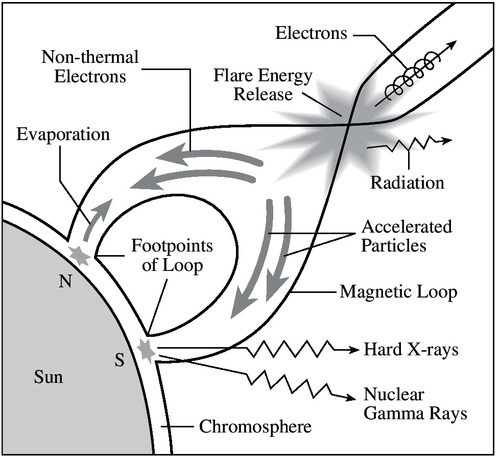
\includegraphics{figures/solar-flare-model.jpg}

        \scriptsize Fig. 1. Solar Flare Model\\
        \scriptsize Source: K.R. Lang, Tufts University, 2010.
    \end{center}
}

%----------------------------------------------------------------------------------------
%	OBJETIVOS
%----------------------------------------------------------------------------------------



\headerbox{Objectives}{name=objectives,span=1,column=0,below=introduction}
{The general objective was to visualize the presence or absence of chromospheric evaporation in spectra
    generated from the analysis of metric radio emission data of a chosen event, and was accomplished
    by first achieving the following specific objectives:
    \begin{itemize}
        \setlength\itemsep{0.01mm}
        \item Data selection and analysis of the chosen event using software that we developed
        \item Comparison of resulting spectra with spectra of other instances of chromospheric evaporation
        \item Discussion about whether the chosen event showed the occurrence of chromospheric evaporation
            on metric radio emissions
    \end{itemize}

}

%----------------------------------------------------------------------------------------
%	METODOLOGIA
%----------------------------------------------------------------------------------------
\headerbox{Methodology}{name=methodology,span=1,column=1,row=0}
{The occurrence of chromospheric evaporation, associated with a X1.0 solar flare
    that took place on March 29, 2014, at the solar active region NOAA AR 12017,
    was visualized in line profile data gathered by the IRIS and EIS spectrographs.
    That line profile data was obtained at multiple times: during the flare’s rise
    (~17:30 UT), during its peak (17:48 UT), and during its decay (~17:54 UT).
    In this present study we analyze the metric radio emission counterpart of that
    same flare, at the same rise, peak and decay times, associated with the chromospheric
    evaporation phenomenon. The radio emission was recorded in the metric (200 --- 450 MHz)
    range by the e-Callisto (Compound Astronomical Low cost Low frequency Instrument for
    Spectroscopy and Transportable Observatory) International Network of Solar Radio Spectrometers,
    and analyzed with scientific computing tools developed by the authors, which are freely available online.
    For comparison, the spectrum of the occurrence of chromospheric evaporation on February 16, 2011,
    during an M1.6 flare (Gömöry et al. 2016), was also generated with the same computational tools, as well as
    the spectrum showing the chromospheric evaporation that happened among a X6.9 flare on August 9, 2011,
    that we had studied previously.
}

%----------------------------------------------------------------------------------------
%	RESULTADO
%----------------------------------------------------------------------------------------
\headerbox{Results}{name=results,span=1,column=1,below=methodology}
{After using the computational tools to analyze the metric radio emission from the selected events,
    the following spectra were obtained:
\begin{center}
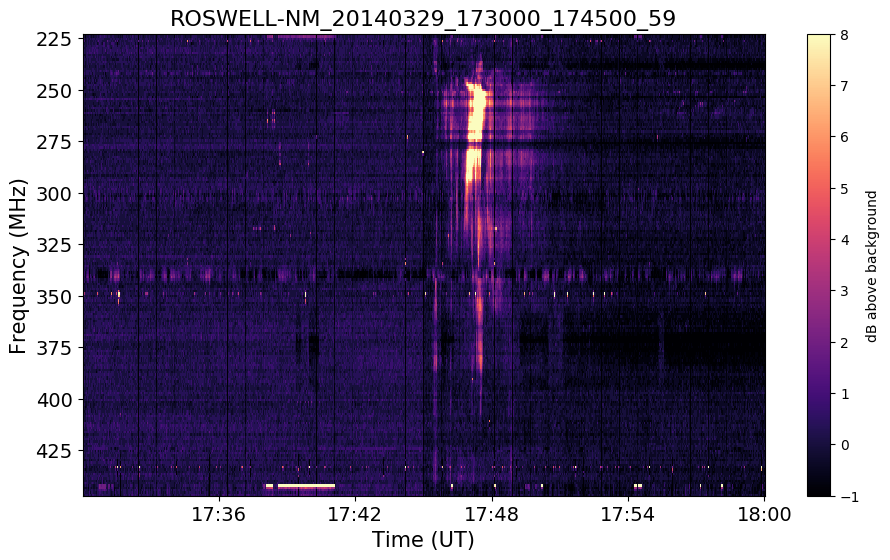
\includegraphics[height=3cm, keepaspectratio]{figures/ROSWELL-NM.png}\\
\tiny(a)

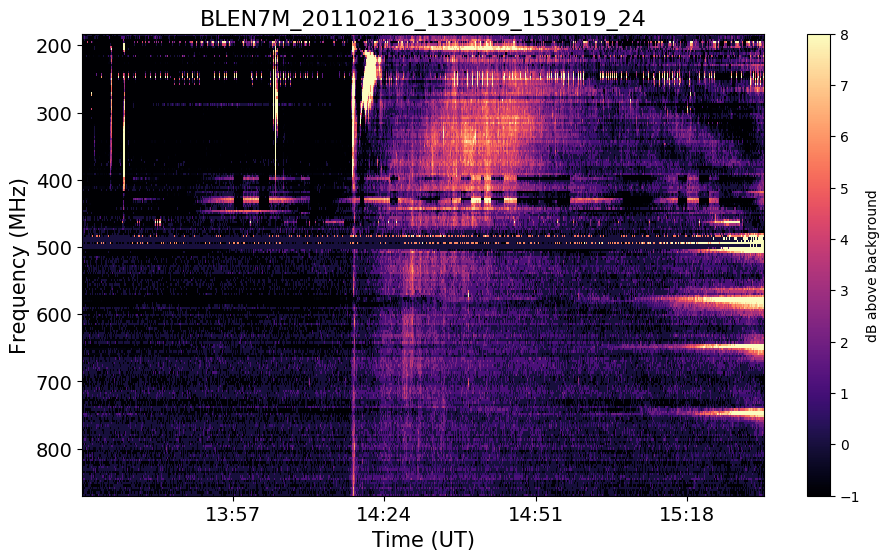
\includegraphics[height=3cm, keepaspectratio]{figures/BLEN7M_20110216.png}\\
\tiny(b)

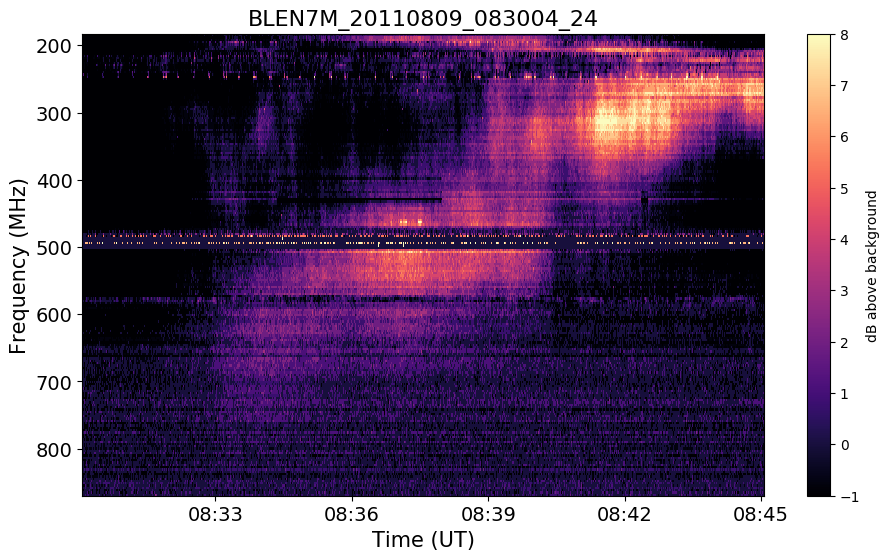
\includegraphics[height=3cm, keepaspectratio]{figures/BLEN7M_20110809.png}\\
\tiny(c)

\scriptsize Fig. 2. Solar radio emission spectrum of data recorded on (a) March 29, 2014 (X1.0 flare),
on (b) February 16, 2011 (M1.6 flare), and on (c) August 9, 2011 (X6.9 flare)

\scriptsize Source: The Authors.
\end{center}

}

%----------------------------------------------------------------------------------------
%	DISCUSSÃO
%----------------------------------------------------------------------------------------
\headerbox{Conclusions}{name=conclusions,column=2,row=0} % To reduce this block to 1 column width, remove 'span=2'
{After selecting which events to compare the March 29, 2014 flare to, we were able to generate solar radio emission
    spectra for all the three events. The generation of these spectra was possible due to the easy access to solar
    spectrometers' data provided in FITS files by the e-Callisto network, and to the fine-tuning of our data analysis
    and visualization tools that came with the observation of multiple events.
    By analyzing and comparing the generated spectra, it is possible to conclude
    that the 2014 flare we chose to study did not show the occurence of chromospheric evaporation on metric radio
    emission data. That is because differently than both the 2011 flares we chose to analyze, it did not present
    a slow drift rate towards lower frequencies, which is characteristic to observations of chromospheric evaporation
    based on metric emissions. This absence of evidence of chromospheric evaporation on the metric emission data we
    analyzed, is possibly related to the fact that the metric emission data is limited by the time cadence and
    spatial resolution of the spectrometers, as stated by Li et.al (2015). And the fact that the IRIS and the EIS,
    used by the same study just mentioned, both have high temporal and spatial resolution, as well as high sensitivity
    in detecting high temperature emissions, could explain why they were able to confirm the occurrence of chromospheric
    evaporation with their line profile data. Nonetheless, our observations are still important since metric radio emission
    data of that event had not been studied before, neither compared to the results obtained by the previously reported
    study of line profile data.
}

%----------------------------------------------------------------------------------------
%	AGRADECIMENTOS
%----------------------------------------------------------------------------------------
\headerbox{Acknowledgements}{name=acknowledgements,column=2,below=conclusions,span=1}
{A.R. Korol would like to thank PIBIC-Univap for his CNPq scientific initiation grant.\\
    F.C.R. Fernandes thanks FAPESP (Proc. 2017/02806--3) and CNPq (Proc. 311376/2015--0).\\
    Both the authors are thankful to the Institute for Data Science FHNW Brugg/Windisch, Switzerland,
    for the data that is freely available on the e-Callisto network.
}

%----------------------------------------------------------------------------------------
%	REFERENCIAS
%----------------------------------------------------------------------------------------
\headerbox{References}{name=references,column=2,below=acknowledgements,span=1}
{[1] Li, Y., et al. 2015, ApJ, 811, 7

[2] De Pontieu, B., Title, A. M., Lemen, J. R., et al. 2014, SoPh, 289, 2733

[3] Culhane, J. L., Harra, L. K., James, A. M., et al. 2007, SoPh, 243, 19

[4] Aschwanden, M. J., Benz, A. O. 1995, ApJ, 438, 997–1012

[5] Sturrock, P. A. 1973, Bull. American Astron. Soc., 5, 280

[6] Gömöry, P., et al. 2016, A\&A, 588, A6

}

%----------------------------------------------------------------------------------------
%	REALIZAÇÃO
%----------------------------------------------------------------------------------------

\headerbox{Realization}{name=event,column=0,below=references, above=bottom,span=3}
{\begin{center}
    
\includegraphics[width=0.7\textwidth]{rodape_simfast.png}
\end{center}
}


\end{poster}

\end{document}
